\documentclass[margin=10pt]{standalone}

\usepackage{tikz}

\usetikzlibrary{decorations.pathreplacing,arrows,shapes,positioning,shadows,calc}

\begin{document}

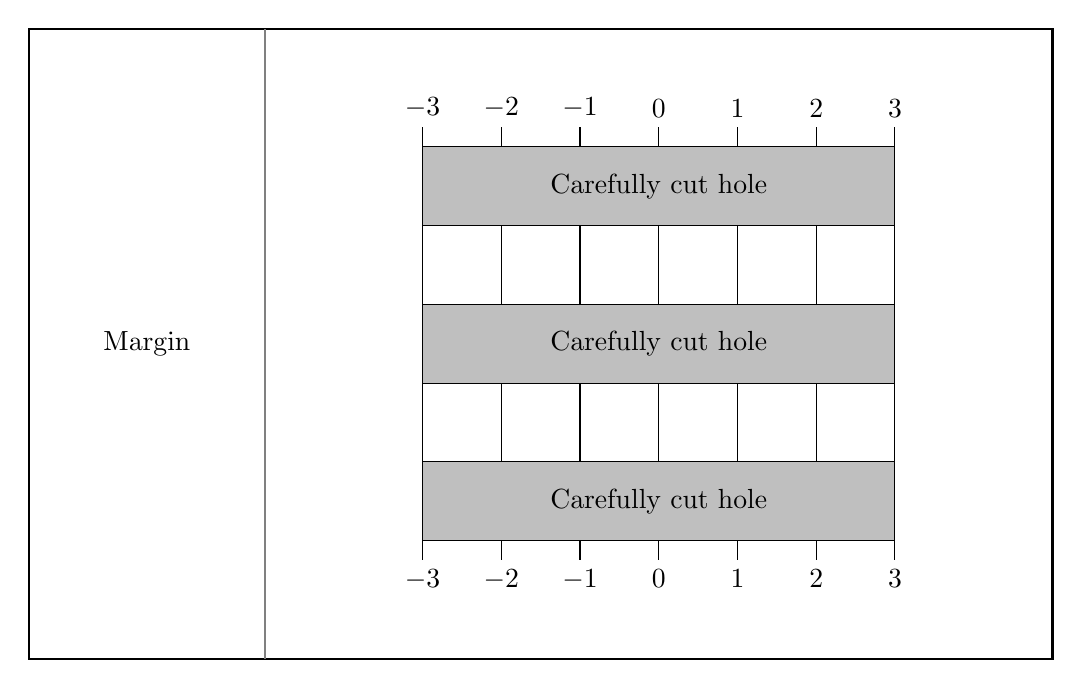
\begin{tikzpicture}
	\draw[thick] (0,0) rectangle (13,8);
	
	\draw[gray] (3,0) -- (3,8);
	\draw (1.5,4) node[anchor=center] {Margin};
	
	\draw (5,1.5) -- ++ (0,-0.25) node[anchor=north] {$-3$};
	\draw (6,1.5) -- ++ (0,-0.25) node[anchor=north] {$-2$};
	\draw (7,1.5) -- ++ (0,-0.25) node[anchor=north] {$-1$};
	\draw (8,1.5) -- ++ (0,-0.25) node[anchor=north] {$0$};
	\draw (9,1.5) -- ++ (0,-0.25) node[anchor=north] {$1$};
	\draw (10,1.5) -- ++ (0,-0.25) node[anchor=north] {$2$};
	\draw (11,1.5) -- ++ (0,-0.25) node[anchor=north] {$3$};

	\draw (5,6.5) -- ++ (0,0.25) node[anchor=south] {$-3$};
	\draw (6,6.5) -- ++ (0,0.25) node[anchor=south] {$-2$};
	\draw (7,6.5) -- ++ (0,0.25) node[anchor=south] {$-1$};
	\draw (8,6.5) -- ++ (0,0.25) node[anchor=south] {$0$};
	\draw (9,6.5) -- ++ (0,0.25) node[anchor=south] {$1$};
	\draw (10,6.5) -- ++ (0,0.25) node[anchor=south] {$2$};
	\draw (11,6.5) -- ++ (0,0.25) node[anchor=south] {$3$};
	
	\draw (5,1.5) -- ++ (0,4);
	\draw (6,1.5) -- ++ (0,4);
	\draw (7,1.5) -- ++ (0,4);
	\draw (8,1.5) -- ++ (0,4);
	\draw (9,1.5) -- ++ (0,4);
	\draw (10,1.5) -- ++ (0,4);
	\draw (11,1.5) -- ++ (0,4);
	

	\draw[fill=lightgray] (5,1.5) rectangle (11,2.5);
	\draw (8,2) node[anchor=center] {Carefully cut hole};
	
	\draw[fill=lightgray] (5,3.5) rectangle (11,4.5);
	\draw (8,4) node[anchor=center] {Carefully cut hole};

	\draw[fill=lightgray] (5,5.5) rectangle (11,6.5);
	\draw (8,6) node[anchor=center] {Carefully cut hole};


\end{tikzpicture}

\end{document}